\documentclass[20pt, a1paper, landscape, margin=0mm, innermargin=8mm,
               blockverticalspace=4mm, colspace=10mm, subcolspace=5mm]{tikzposter}

\usepackage[utf8]{inputenc}
\usepackage[T1]{fontenc}
\usepackage{lmodern}
\usepackage{graphicx}
\usepackage{xcolor}
\usepackage{array}
\usepackage{hyperref}
\usepackage{enumitem}

\tikzposterlatexaffectionproofoff

% --- palette ---------------------------------------------------------------
\definecolor{ink}{HTML}{222222}
\definecolor{muted}{HTML}{6E8E8A}
\definecolor{mutedlight}{HTML}{B5C9C6}
\definecolor{cool}{HTML}{4F7A8A}
\definecolor{warm}{HTML}{D9A441}
\definecolor{bad}{HTML}{B5584D}
\definecolor{bg}{HTML}{FAFAFA}
\definecolor{panelbg}{HTML}{FFFFFF}
\definecolor{notebg}{HTML}{F1EFE6}

% --- theme -----------------------------------------------------------------
\usetheme{Simple}
\definebackgroundstyle{soft}{
  \draw[fill=bg,draw=none] (bottomleft) rectangle (topright);
}
\usebackgroundstyle{soft}

\defineblockstyle{TightBar}{
  titlewidthscale=1, bodywidthscale=1, titlecenter,
  titleoffsetx=0pt, titleoffsety=0pt, bodyoffsetx=0pt, bodyoffsety=0pt,
  bodyverticalshift=0pt, roundedcorners=0, linewidth=0.5pt,
  titleinnersep=8pt, bodyinnersep=9pt
}{
  \draw[color=framecolor, fill=blockbodybgcolor, line width=\blocklinewidth]
    (blockbody.south west) rectangle (blockbody.north east);
  \ifBlockHasTitle
    \draw[color=blocktitlebgcolor, fill=blocktitlebgcolor, line width=0pt]
      (blocktitle.south west) rectangle (blocktitle.north east);
  \fi
}
\useblockstyle{TightBar}
\colorlet{blocktitlebgcolor}{muted}
\colorlet{blocktitlefgcolor}{white}
\colorlet{blockbodybgcolor}{panelbg}
\colorlet{blockbodyfgcolor}{ink}
\colorlet{framecolor}{muted}
\colorlet{backgroundcolor}{bg}
\colorlet{titlebgcolor}{bg}
\colorlet{titlefgcolor}{ink}

\setlist[itemize]{leftmargin=*, itemsep=0pt, topsep=0pt, parsep=1pt}
\setlist[enumerate]{leftmargin=*, itemsep=0pt, topsep=0pt, parsep=1pt}

\title{\parbox{0.96\linewidth}{\centering Tokenization for Noisy Texts: An Empirical Study on Named Entity Recognition}}
\author{Alexander Malyy}
\institute{Innopolis University \quad\textbar\quad NLP (S26) \quad\textbar\quad Case Study 1.7}

\makeatletter
\settitle{
  \centering
  \begin{minipage}{0.96\linewidth}
    \centering
    \color{titlefgcolor}{\bfseries \Huge \@title}\\[0.3em]
    {\Large \@author} \\[0.1em]
    {\normalsize \color{muted} \@institute}
  \end{minipage}
}
\makeatother

\newcommand{\headline}[2]{%
  \begin{minipage}{0.95\linewidth}\centering
    {\color{warm}\fontsize{28}{32}\selectfont\bfseries #1}\\[-2pt]
    {\footnotesize #2}
  \end{minipage}\par\vspace{3pt}
}

\newcommand{\callout}[1]{{\color{cool}\textbf{#1}}}
\newcommand{\warm}[1]{{\color{warm}\textbf{#1}}}
\newcommand{\brd}[1]{{\color{bad}\textbf{#1}}}

\begin{document}
\maketitle[width=0.96\linewidth, roundedcorners=0, linewidth=0pt, innersep=8pt,
          titletotopverticalspace=-12pt, titletoblockverticalspace=8pt]

\begin{columns}

% =========== LEFT COLUMN (narrow, text-heavy) ==============================
\column{0.24}

\block{Motivation \& questions}{
Real-world text is noisy before any NLP model sees it: \textbf{OCR} errors,
\textbf{ASR} transcripts without casing or punctuation, \textbf{social-media}
abbreviations and typos. Tokenization is the first step of every modern pipeline;
modern subword/byte-level tokenizers avoid OOV by construction \,---\, but do they
stay \emph{stable} under noise?
\smallskip

\textbf{RQs:} (1) How does noise perturb tokenization (fertility, token drift)?
(2) Which tokenizer family (WordPiece / BPE / byte-level) is most noise-robust?
(3) Can inference-time preprocessing or noisy fine-tuning recover NER F1, and
which works when?
}

\block{Experimental setup}{
\textbf{Dataset:} CoNLL-2003 English NER, 3{,}453 test sents, entity-level
seqeval F1.\\[2pt]
\textbf{Models} (tokenizer / vocab / F1 on clean):\\[1pt]
\begin{tabular}{@{}lll@{}}
  bert-base-uncased & WordPiece / 30.5K  & 0.89 \\
  bert-base-cased   & WordPiece / 28.9K  & 0.90 \\
  gpt2              & BPE / 50.2K        & 0.69 \\
  byt5-small        & byte / 256         & 0.86 \\
\end{tabular}\\[4pt]
\textbf{Noise} ($p{=}0.3$/tok): OCR visual confusions, ASR lowercase+phonetic,
social typos+abbrev (Belinkov \& Bisk, TextFlint).\\[2pt]
\textbf{Interventions:} rule-based per-channel \emph{preprocess} (word-count
preserving) + mixed-noise \emph{fine-tune} (1 epoch, 50\% clean / 50\% noise).
}

\block{Key results (mean across 12 model-noise cells)}{
\centering
\renewcommand{\arraystretch}{1.05}
\begin{tabular}{@{}lcc@{}}
\hline
                              & \textbf{mean F1} & \textbf{\% recovery} \\
\hline
Clean baseline                & \textbf{0.83} & \,---\, \\
Noisy (no mitigation)         & 0.55 ($-0.28$) & 0\% \\
+ inference preprocess        & 0.69          & 49\% \\
+ noisy fine-tune             & 0.69          & 47\% \\
Best per cell                 & \textbf{0.71} & \textbf{55\%} \\
\hline
\end{tabular}\\[4pt]
\raggedright\footnotesize
Either intervention alone recovers $\approx$ half the noise gap; best-per-cell adds $+0.02$ over the winner. Neither fully closes the $0.28$ drop.
}

\block{Conclusions}{
\begin{itemize}
\item ``No UNK'' $\neq$ noise-robust. Coverage = fertility inflation + token drift. Byte-level helps tokenizer layer, not F1 layer.
\item Single component dominates per channel (truecase / ASR, charfix / OCR, spellcheck / social) \,---\, target, don't uniformly preprocess.
\item Preprocess vs fine-tune = per-cell tradeoff; both act via
\textbf{token stability} (causal lever, $r{=}0.88$).
\end{itemize}
}

% =========== CENTER COLUMN (plots) =========================================
\column{0.40}

\block{Tokenizer fertility: clean $\to$ noisy $\to$ preprocess}{
\centering
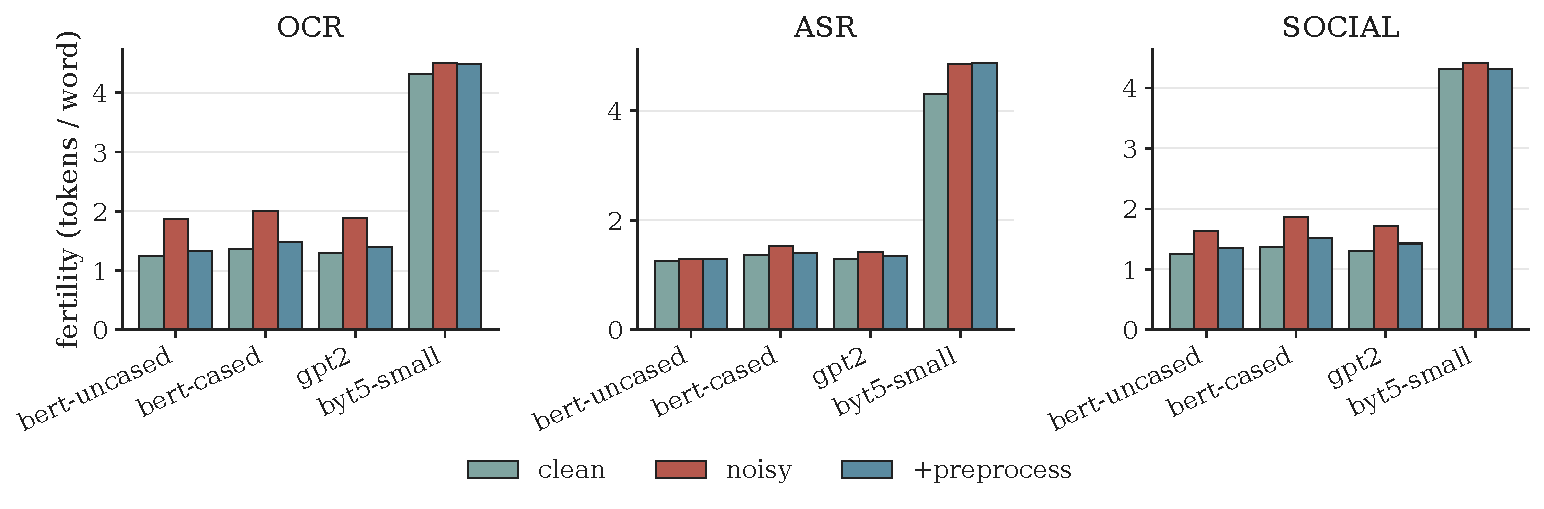
\includegraphics[width=0.98\linewidth]{figures/fertility_3panel.pdf}\\[1pt]
\raggedright\small
Subword tokenizers fragment heavily under OCR (\brd{+45\% to +50\%} tokens/word).
Byte-level is structurally noise-robust (\callout{+2\% social, +4\% OCR, +12\% ASR}). Preprocess restores
fertility close to clean on OCR/social; ASR is modest (phonetic swaps produce
in-vocab words).
}

\block{Token-set stability: Jaccard vs clean reference}{
\centering
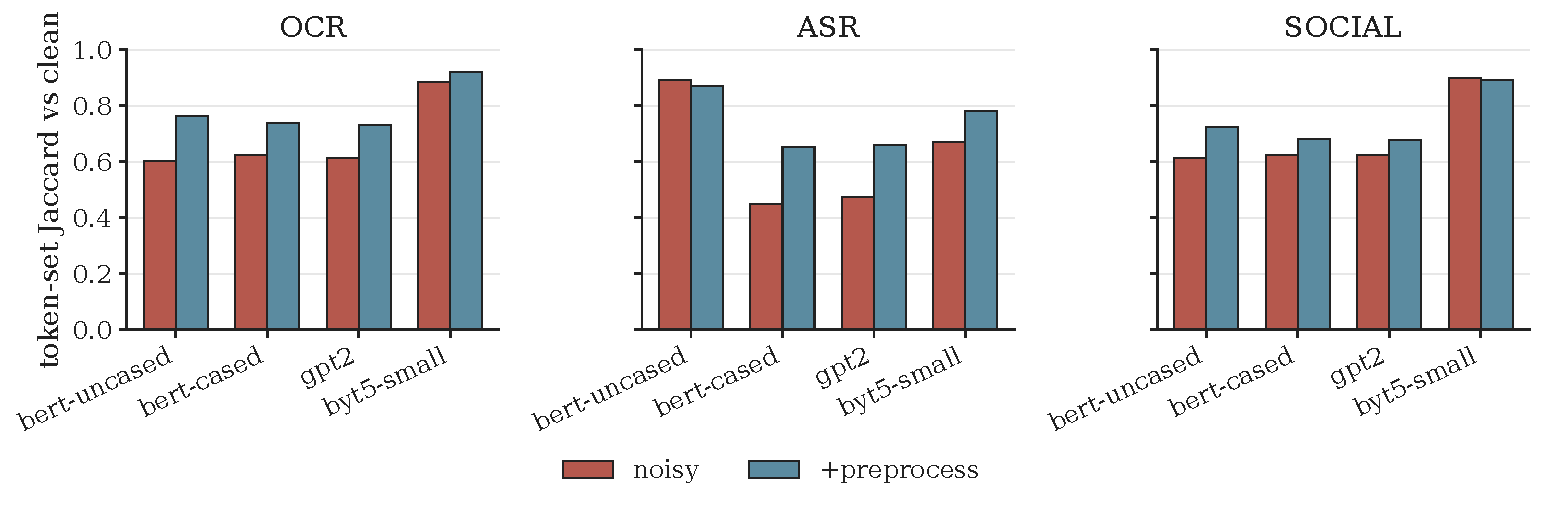
\includegraphics[width=0.98\linewidth]{figures/overlap_3panel.pdf}\\[1pt]
\raggedright\small
ASR scrambles \emph{cased} tokenizer outputs most (Jaccard to \brd{0.45-0.48});
truecasing recovers \callout{half}. ByT5 stays $\geq 0.67$ across all channels.
}

\block{Mitigation matrix: F1 per (model, noise) $\times$ intervention}{
\centering
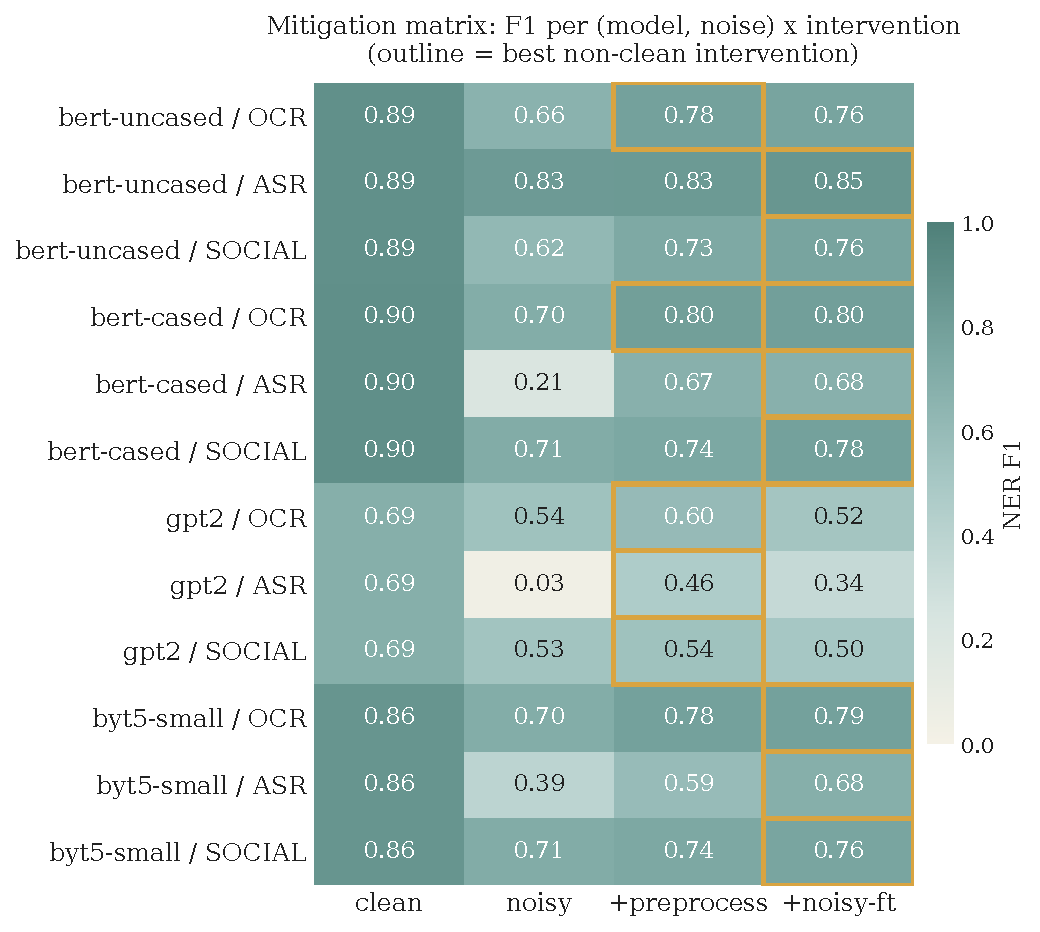
\includegraphics[width=0.82\linewidth]{figures/f1_heatmap.pdf}\\[1pt]
\raggedright\small
\textbf{No universal winner.} Preprocess wins all gpt2 cells; noisy-fine-tune
wins byt5 and 2/3 bert-uncased; the two \emph{split} on bert-cased. ASR rows are
darkest under noise (\brd{0.03 gpt2, 0.21 bert-cased}) and lighten most under
either intervention (outline = best non-clean intervention per row).
}

% =========== RIGHT COLUMN ==================================================
\column{0.30}

\block{Preprocessing pipeline (per channel)}{
\small
\renewcommand{\arraystretch}{1.2}
\setlength{\tabcolsep}{6pt}
\begin{tabular}{@{}lll@{}}
\textbf{Channel} & \textbf{Pipeline} & \textbf{Example} \\
\hline
OCR    & \warm{char-fix} $\to$ \warm{spellcheck}                         & \texttt{hel1o}  $\to$ \texttt{hello} \\
ASR    & \warm{truecase} $\to$ \warm{homophone-fix}                      & \texttt{ur}     $\to$ \texttt{your}  \\
Social & \warm{un-repeat} $\to$ \warm{un-abbrev} $\to$ \warm{spellcheck} & \texttt{gr8}    $\to$ \texttt{great} \\
\end{tabular}\par\smallskip
{\footnotesize \textbf{Word-count preserving} \,---\, no splits, merges, or insertions. BIO labels stay aligned during NER eval. Spellcheck: pyspellchecker, edit-distance 1.}
}

\block{Which preprocessing component matters?}{
\centering
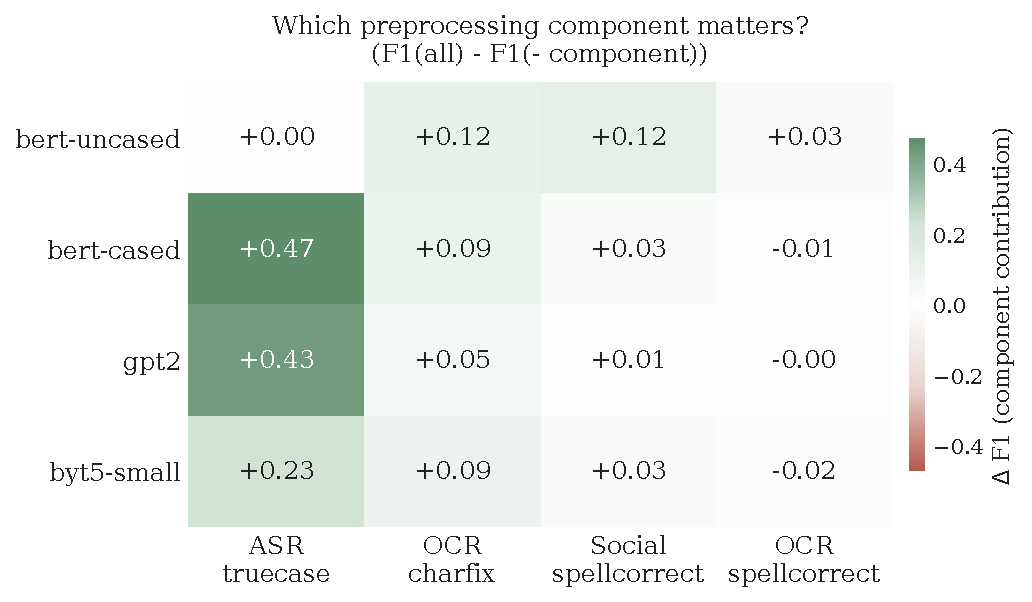
\includegraphics[width=0.98\linewidth]{figures/ablation_heatmap.pdf}\\[1pt]
\raggedright\small
ASR \warm{truecase} is life-saving for cased models (\warm{+0.47} bert-cased, \warm{+0.43} gpt2). OCR \warm{charfix} dominates char-level recovery. OCR spell-correct \textbf{overcorrects} on cased/byte models (rewrites rare entities).
}

\block{Mechanism: tokenization stability predicts F1}{
\centering
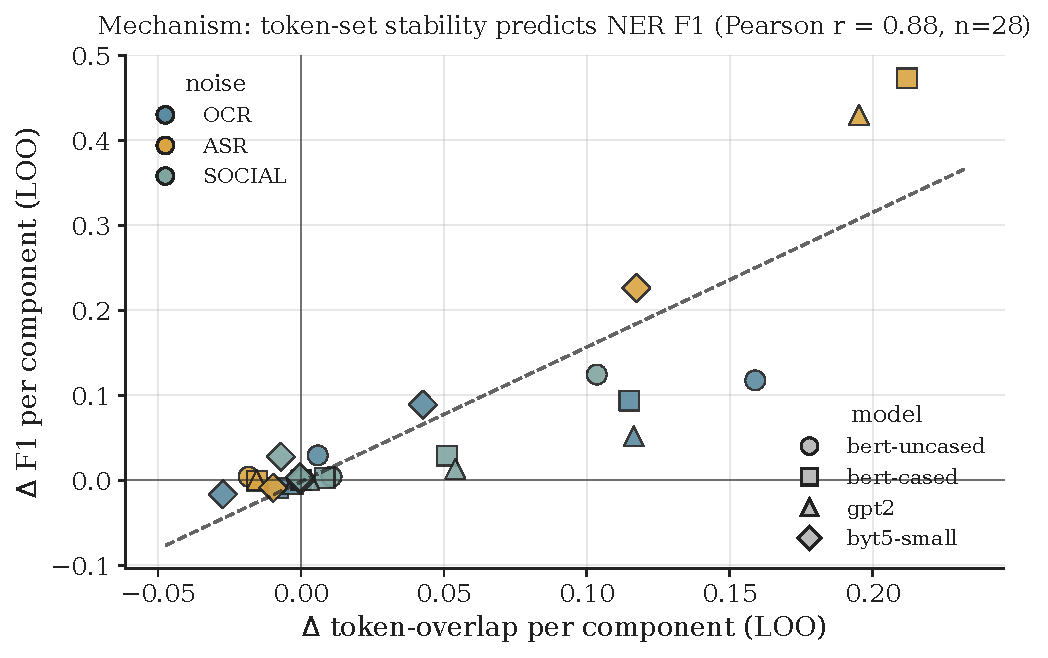
\includegraphics[width=0.98\linewidth]{figures/mechanism_scatter.pdf}\\[1pt]
\raggedright\small
Across \callout{28 LOO component cells}, F1 contribution is strongly predicted by token-set stability change (\warm{Pearson $r=0.88$}) \,---\, components that bring tokenization closer to clean recover NER F1.
}

\block{Limitations \& code}{
\footnotesize
\textbf{Limits:} 1-epoch training; rule-based preprocess (no contextual MLM); punct-restore out-of-scope (BIO); English NER only; gpt2 clean F1 low (0.69) \,---\, absolute cross-model comparisons skew. Refs (Belinkov\&Bisk, TextFlint, CoNLL, seqeval) in repo README.\\[1pt]
\textbf{Code:} \texttt{github.com/n4rly-boop/S26-NLP-Tokenization-for-Noisy-Texts}
}

\end{columns}

\end{document}
